% !TeX root = ../main.tex
% Add the above to each chapter to make compiling the PDF easier in some editors.

\chapter{Introduction}\label{chapter:introduction}
Peer review is the formal process of the evaluation of scholarly works by people specialized in the subject of the work \parencite[p.~864]{Moxham.2018}. Common applications of peer review in scientific research are the selection of grant and fellowship applications, and the selection of manuscripts for scientific journals. In academic publishing when a researcher submits an academic paper for publication, journal editors ask “peers”, who are experts in the field to scrutinize the paper. Based on these reports the editor either rejects the paper, sends the paper back to the author for revision, or accepts it for publication. By determining what gets published or who gets funding, reviewers act as gatekeepers of science and the process ensures the quality and soundness of the scientific work \parencite{Bornmann.2011}.

\begin{figure}[htpb]
  \centering
  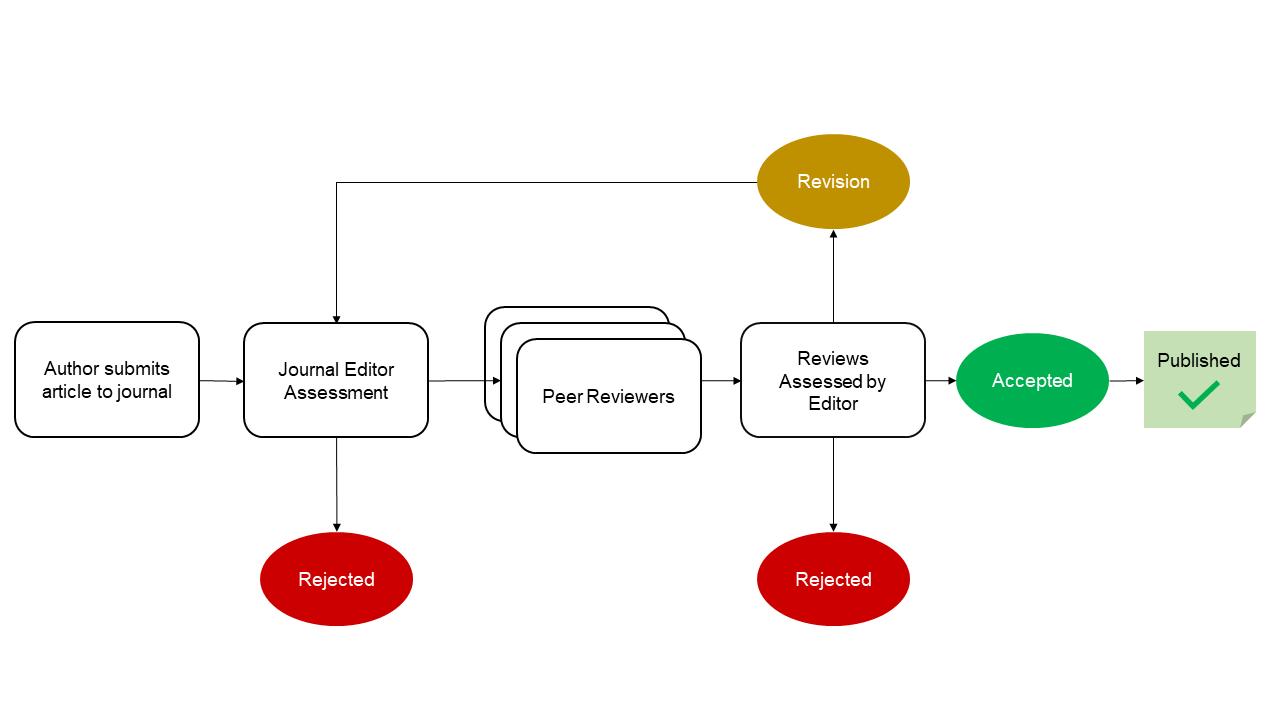
\includegraphics[width=0.8\textwidth]{figures/publishing-process.png}
  \caption{The publishing process} \label{fig:publishing-process}
\end{figure}

Peer reviews can be classified by which parties know the identities of others. In a double-blind review, only the editor knows the identities of the author and the reviewer. In a single-blind review, the name of the reviewer is hidden from the author to let the reviewer criticize without worrying about personal relationships or conflict of interests. The third and emergent form of the peer re-view is open peer review where the identities of both author and the reviewer are known to each other. In some forms of the open peer review, the identities and the review reports are also publicly available \parencite[4]{HorbachS.P.J.M..2017}, and therefore reviewers can gain credit for their work. 

Nevertheless, peer review takes place in many different forms and employs different process-es and it’s difficult to acknowledge it as a single system \parencite[2]{HorbachS.P.J.M..2017}. But its essence and rationale are shared among all different applications. Emerged among earlier scientific societies as an internal scrutinization for the scientific quality of manuscripts, it held its importance throughout the proliferation of the printing press, globalization of science after World War II \parencite{Fyfe.2017}, and the adoption of information technologies. It is still perceived by some as the gold standard in scientific publishing \parencite{Mayden.2012} and provides legitimacy for the generated knowledge \parencite{Tennant.2020c}.


\section{Problem Statement}

It is widely accepted that peer review plays an important role in research \parencite{Publons.2018, Taylor&Francis.2015, Ware.2008, Zuckerman.1971}. Despite its importance, peer review is shown to be far from being perfect, by being prone to biases \parencite{Lee.2013, Mahoney.1977}, inconsistencies \parencite{Peters.1982, Rothwell.2000}, and being ineffective in detecting errors \parencite{Schroter.2004}. It usually takes 3 to 5 hours (\cite[146]{Mulligan.2013}; \cite[42]{Ware.2008}) to complete a review and it usually takes more than 3 months for a paper to be accepted \parencite[51]{Ware.2008}. The process is often slow for authors and time consuming for reviewers. Reviewers who are academics themselves with various duties are often not compensated for their review work and they don’t receive credit for their work. Given that number of publications is growing each year \parencite{Bornmann.2015} and each manuscript typically requires 2 to 3 reviewers the peer review system is being put under growing pressure. This situation is said to cause “reviewer fatigue” \parencite{Breuning.2015}. At the same time, editors are reporting that it is getting more difficult to find suitable reviewers, indicated by the increasing decline rates to review invitations \parencite{Baveye.2011, Fox.2017}. 

Despite the numerous deficiencies of the process, it is argued that there is no consensus on an alternative \parencite{Smith.2006, Young.2003} and it is currently the best method ensuring the soundness of scientific publishing (\cite[5201]{Grainger.2007}; \cite[2]{HorbachS.P.J.M..2017}). A range of innovations aimed to tackle the stated problems failed to provide a cure and the peer review remains mostly unchanged \parencite{Tennant.2017}. 


\subsubsection{Peer Review Lacks Incentives}

Some of the problems of peer review are believed to be results of the lack of incentives to review \parencite{Derraik.2015, Willis.2016}, and a there’s an ongoing discussion on how to increase researchers’ engagement in reviews in the light of these problems \parencite{Derraik.2015, Gasparyan.2015, Hauser.2007, Squazzoni.2013}. The lack of incentives has its roots within that today the measures and indicators of academic performance are the number of papers published, number of citations, or other citation based scientometrics. These measures play an important role in deciding who climbs up the ranks, who gets hired, or who receives the funding. Despite its importance, peer reviews usually are not recognized as a research output as the manuscripts and do not contribute to researchers’ perceived academic performance \parencite{Tennant.2017}. Therefore, researchers are disincentivized to do reviews and incentivized to publish more manuscripts.

The reliance on publishing-related metrics has also other consequences on peer reviewing. The state of affairs creates the mindset of “publish or perish”: the constant pressure to publish more and get cited more \parencite{Rawat.2014}. Yet, the way to publish more and get cited more is not only doing more research. One can publish the results of their work in smaller and less coherent slices \parencite[4]{Ferreira.2016} in an act called “salami publication” \parencite{SupakSmolcic.2013} (Supak Smolcić, 2013). The act is considered unethical \parencite[238]{SupakSmolcic.2013} and with each paper reviewed by multiple reviewers, it puts more pressure on the peer review system \parencite[4]{Ferreira.2016}. This effect is amplified when a paper gets redundantly reviewed in different journals i.e. when authors go “journal shopping”. In this case, following a rejection by a journal with a higher impact, authors continue submitting their papers to gradually lower impact journals until their papers get published while the new editors and reviewers of the submitted paper are not aware of the previous reviews done \parencite[10]{Kovanis.2016}. 

If everyone publishes more and reviews less, then who is doing all the reviews? A strong imbalance in the peer review system was observed where a larger percentage of the peer reviews are done by a minority of researchers and thanks to them there is a sufficient supply of reviewers (\cite{Kovanis.2016}; \cite{Petchey.2014}; \cite[37]{Ware.2008}). Those “peer-review heroes” bear the burden by reviewing much more than they publish \parencite[9]{Kovanis.2016}. The situation raises the concerns that the system may be in a “tragedy of the reviewer commons” \parencite{Hochberg.2009} where participants of the system are encouraged to exploit the system by submitting more papers and less incentivized to do peer reviews. 

There’s a consensus among researchers that an improvement in peer review incentives would enable better reviews \parencite{Publons.2018}. Attracting more reviewers to the reviewer pool would also help balance the heavy burden placed on the reviewing system potentially letting editors find reviewers easier and shorten the time taken from submission until the publication of a manuscript. 

\subsubsection{Closedness of Reviews Prevents Its Acknowledgment}

The practice of blinded reviewing is a feature of the process that hinders public review acknowledgement. Today most of the peer reviews are done as single or double-blind \parencite{Wolfram.2020}. Even though open peer review seems to be gaining popularity \parencite{Wolfram.2020}, scientists are more likely to accept review requests when their identities are hidden \parencite{vanRooyen.1999} and majority of the researchers still prefer blinded reviews over open peer reviews (\cite[149]{Mulligan.2013}; \cite{Taylor&Francis.2015}; \cite[1038-1039]{Wolfram.2020}). It is likely the majority of peer reviews will remain blinded as the anonymity is considered necessary for strong and unbiased scrutiny \parencite[21-23]{RossHellauer.2017}.

However, a problem the closedness of reviews introduces is the difficulty to verify reviews. Since the whole review process takes place internally in journal management systems it is not possible to find out externally if a researcher has really done a peer review for a specific manuscript or a journal, without explicitly contacting the journal. In most of the cases, the transaction costs of contacting a journal is too large for a review, as virtually none of the journals has such a verification system. For reviewers to gain recognition for their work, it is essential that they can easily prove the authenticity of their reviews. The researchers may then showcase their review works done for specific journals and articles publicly or present them when needed as a demonstration of expertise in a field e.g. in job and grant applications. It may also high-light the reviewing workloads of researchers to their employers \parencite[2]{Raoult.2020}. 

Employers are increasingly resorting more to citation-based metrics for assessing their researchers \parencite{Bianchi.2019, Cantor.2015, Kachewar.2013, Verissimo.2013}. These metrics may be taken into account when assessing academic performance \parencite[11]{Ferreira.2016}. Availability of peer review contributions or related metrics may also bring incentives to do more reviews and reduce the imbalance in the review workloads \parencite[4]{Petchey.2014}. 

\subsubsection{Existing Peer Review Recognition Platforms Are Becoming the Sole Owners of Peer Review Data}

There are already running projects that aim to incentivize peer reviews by letting reviewers showcase their work. The unavailability of the peer review data and the inability to verify reviews lead to the provision of review acknowledgment by external services where these platforms verify the authenticity of reviews and act as trusted third parties between reviewers and the bodies potentially interested in this information such as editors, funders, universities or agencies.

Reviewer Credits \footnote{https://www.reviewercredits.com/}  is a project to let reviewers certify peer review activity, display their review records, and earn rewards such as books, and discounts to paid publishing services. Reviewers can claim their activity either through automated data transfer between the platform and journal or by Reviewer Credits manually contacting the publisher. The more popular platform providing a similar service is Publons. Founded by Andrew Preston and Daniel Johnston in New Zealand in 2012 it quickly gained popularity and was welcomed by many academics \parencite[266]{Smith.2015} and was eventually acquired by Clarivate Analytics in 2017. As of November 2020, Publons claims to have over 2 million members\footnote{http://web.archive.org/web/20201109015743/https://publons.com/about/home}. On Publons, researchers can create a profile and add the reviews they have done. To add a peer review, they can either follow a link provided by the journal with a Publons integration after submitting their review or they can manually forward their review acceptance emails to Publons, who then manually verifies the review. By gathering publications and reviews, researchers can showcase their scholarly efforts and earn badges and awards such as “Top Reviewer” or “Highly Cited”. 

Despite the acceptance of the platform, it’s pointed out how it may be failing to distinguish authentic reviews \parencite{TeixeiradaSilva.2020} and that its metrics may be biased \parencite{Ortega.2017}. Besides, the fact that the data on the platform is owned by Publons, and effectively Clarivate Analytics, brings the accessibility of the data into question. The platform’s provided API does not provide much data and existing studies making use of the Publons data extract it using web crawlers \parencite[952]{Ortega.2017} which is not allowed without Publons’ written consent according to the platform’s terms\footnote{https://publons.com/about/terms}. However the platform appears to have provided data to researchers when requested \parencite[12]{Kovanis.2016}. Concerns have also been expressed for the transparency of the data previously provided by Clarivate Analytics (\cite{Rossner.2007}; \cite[3]{TeixeiradaSilva.2019}), as the provider of the Journal Impact Factor, and for the fairness of its practices \parencite{TeixeiradaSilva.2013}.

The centralization in scientific publishing, through acquisitions of journals, has paved the way for oligopolistic behavior in publishers \parencite{Lariviere.2015}. By bundling journals and employing price discrimination for different institutes, for-profit publishers are able to sell scientific publications at much higher costs than nonprofits \parencite{Bergstrom.2014}. Not all institutions can pay the increasing costs to access scientific literature and single access to articles is not affordable for individuals. This causes the accessibility to scientific information and the progress of science to be hindered \parencite[3]{Tennant.2016}. Despite the proliferation of information technologies, which drove the marginal costs for access and circulation of knowledge to negligible levels, the publication costs have been increasing constantly \parencite{Tennant.2016}. The situation brought the role traditional publishers playing and the value they are adding into question \parencite{Heise.2020}. Centralization in the peer review data may introduce similar problems.

The aggregation of peer review data might also be inappropriate for publishers and journals. The journals are effectively giving away their valuable review data to Publons for free. In turn, Clarivate Analytics processes this data and makes use of it for their profit. An example is the editor matching tool Publons has that lets editors find suitable matches for peer reviews of a manuscript\footnote{https://publons.com/benefits/reviewer-connect}. As long as the world’s peer review data is under the control of a single party, there exists the possibility for the sole owner of the data to restrict access to it. With already apparent problems of centralization in publishing \parencite{Lariviere.2015} and ever more demand for open science \parencite[1-3]{Piwowar.2018}, there should be ways to aggregate and process review data that will give its participants the control over their data. 

Additionally, disintermediation of review recognition platforms as verifiers may enable a range of experiments on peer review incentivization. Attempts to incentivize peer review need to assume open peer reviews or keep the domain of the solution small such as a single publisher or a journal. On top of the available decentralized verified peer review data, different incentivization schemes may be built or alternative metrics may be introduced. 

